\documentclass[10pt,a4paper]{scrartcl}

% -----------------------------------------------------------------------------
% PACKAGES & SETUP
% -----------------------------------------------------------------------------
\usepackage[utf8]{inputenc}
\usepackage[T1]{fontenc}
\usepackage{helvet}
\renewcommand{\familydefault}{\sfdefault}
\usepackage{microtype}
\usepackage{amsmath,amssymb}

\usepackage[top=1.4cm, bottom=1.8cm, left=1.5cm, right=1.5cm, headheight=14pt]{geometry}

\usepackage[table]{xcolor}
\definecolor{NavyDark}{HTML}{0A192F}
\definecolor{NavyPrimary}{HTML}{0F2C59}
\definecolor{BlueAccent}{HTML}{1E56A0}
\definecolor{LightBlueBg}{HTML}{F0F4F8}
\definecolor{CardBg}{HTML}{F8FAFC}
\definecolor{BuyGreen}{HTML}{00875A}
\definecolor{TextDark}{HTML}{1E293B}
\definecolor{TextMuted}{HTML}{64748B}
\definecolor{BorderGray}{HTML}{CBD5E1}
\definecolor{BearRed}{HTML}{D97706}

\usepackage{graphicx}
\usepackage{tikz}
\usetikzlibrary{calc,positioning,shapes.geometric,backgrounds}

\usepackage{tabularx}
\usepackage{booktabs}
\usepackage{multirow}
\usepackage{array}
\usepackage[most]{tcolorbox}
\usepackage{enumitem}
\usepackage{fontawesome5}
\usepackage{fancyhdr}
\usepackage[hidelinks]{hyperref}

% Header and Footer Setup
\pagestyle{fancy}
\fancyhf{}
\renewcommand{\headrulewidth}{0.4pt}
\renewcommand{\footrulewidth}{0.4pt}
\fancyhead[L]{\small\textcolor{NavyPrimary}{\textbf{MERIDIAN CAPITAL MARKETS}} \ \vline \ \textcolor{TextMuted}{Institutional Equity Research}}
\fancyhead[R]{\small\textcolor{TextMuted}{July 24, 2026 \ $\cdot$ \ Enterprise Software}}
\fancyfoot[L]{\small\textcolor{TextMuted}{\textbf{Nexa Cloud Solutions Inc. (NXCL)} \ $\cdot$ \ Equity Research Analyst Report}}
\fancyfoot[R]{\small\textcolor{TextMuted}{Page \thepage\ of 3}}

% TColorBox Styles
\tcbset{
    basebox/.style={
        enhanced,
        arc=3pt,
        boxrule=0.8pt,
        fonttitle=\bfseries\sffamily,
        coltitle=white,
        colback=white,
        colframe=NavyPrimary,
        top=6pt, bottom=6pt, left=8pt, right=8pt
    },
    targetbox/.style={
        enhanced,
        arc=4pt,
        boxrule=1pt,
        colback=LightBlueBg,
        colframe=NavyPrimary,
        top=6pt, bottom=6pt, left=8pt, right=8pt
    },
    calloutbox/.style={
        enhanced,
        arc=3pt,
        boxrule=0.6pt,
        colback=CardBg,
        colframe=BorderGray,
        top=6pt, bottom=6pt, left=8pt, right=8pt
    }
}

% Helper column types
\newcolumntype{R}{>{\raggedleft\arraybackslash}X}
\newcolumntype{C}{>{\centering\arraybackslash}X}
\newcolumntype{L}{>{\raggedright\arraybackslash}X}

\begin{document}

% -----------------------------------------------------------------------------
% HEADER BANNER & RATING BOX
% -----------------------------------------------------------------------------
\begin{minipage}[t]{0.67\textwidth}
    \vspace{0pt}
    \textcolor{NavyPrimary}{\Large\textbf{Nexa Cloud Solutions Inc. (Meridex: NXCL)}} \\[3pt]
    \textcolor{NavyDark}{\huge\textbf{Scaling the Next-Gen Enterprise AI Fabric}} \\[6pt]
    \textcolor{TextMuted}{\small\textbf{Initiating coverage with BUY rating and \$245 Target Price driven by multi-year cloud migration tailwinds, proprietary AI orchestration margins, and expanding net expansion rate.}}
\end{minipage}%
\hfill
\begin{minipage}[t]{0.31\textwidth}
    \vspace{0pt}
    \begin{tcolorbox}[targetbox, top=4pt, bottom=4pt, left=6pt, right=6pt]
        \centering
        \small\textcolor{NavyPrimary}{\textbf{INVESTMENT RATING}} \\[2pt]
        {\Huge\textbf{\textcolor{BuyGreen}{BUY}}} \\[4pt]
        \small
        \begin{tabular}{@{}ll@{}}
            \textbf{Target Price:} & \textbf{\$245.00} \\
            Current Price: & \$182.50 \\
            Implied Upside: & \textcolor{BuyGreen}{\textbf{+34.2\%}} \\
            Risk Profile: & Moderate / Core
        \end{tabular}
    \end{tcolorbox}
\end{minipage}

\vspace{8pt}
\hrule height 0.8pt
\vspace{8pt}

% -----------------------------------------------------------------------------
% PAGE 1: KEY DATA & EXECUTIVE SUMMARY
% -----------------------------------------------------------------------------
\begin{minipage}[t]{0.32\textwidth}
    \vspace{0pt}
    \begin{tcolorbox}[calloutbox, title=\textcolor{NavyPrimary}{Market Data Snapshot}, colframe=NavyPrimary, colbacktitle=NavyPrimary, coltitle=white]
        \scriptsize
        \begin{tabular}{@{}lr@{}}
            \textbf{52-Wk High / Low:} & \$195.40 / \$124.10 \\
            \textbf{Market Cap (\$B):} & \$42.85 \\
            \textbf{Enterprise Value (\$B):} & \$40.12 \\
            \textbf{Shares Outstanding (M):} & 234.8 \\
            \textbf{Free Float (\%):} & 88.4\% \\
            \textbf{30D Avg Vol (M):} & 4.15 \\
            \textbf{Dividend Yield (\%):} & 0.0\% \\
            \textbf{Net Debt / EBITDA:} & -1.2x (Net Cash) \\
            \textbf{Beta (3Y Monthly):} & 1.18 \\
            \textbf{Fiscal Year End:} & December 31
        \end{tabular}
    \end{tcolorbox}

    \vspace{4pt}

    \begin{tcolorbox}[calloutbox, title=\textcolor{NavyPrimary}{Research Analysts}, colframe=NavyPrimary, colbacktitle=NavyPrimary, coltitle=white]
        \scriptsize
        \textbf{Alexander Vance, CFA} \\
        \textcolor{TextMuted}{Lead Tech Analyst} \\
        \faEnvelope \ \texttt{a.vance@meridiancap.com} \\[4pt]
        \textbf{Sarah Jenkins} \\
        \textcolor{TextMuted}{Associate Analyst} \\
        \faEnvelope \ \texttt{s.jenkins@meridiancap.com}
    \end{tcolorbox}
\end{minipage}%
\hfill
\begin{minipage}[t]{0.65\textwidth}
    \vspace{0pt}
    \begin{tcolorbox}[calloutbox, title=\textcolor{NavyPrimary}{Executive Summary \& Investment Thesis}, colframe=NavyPrimary, colbacktitle=LightBlueBg, coltitle=NavyPrimary]
        \small
        Nexa Cloud Solutions Inc. (\textbf{NXCL}) has established itself as the leading hybrid enterprise AI orchestration fabric. As Fortune 500 organizations transition from experimental LLM deployments to production-grade distributed architectures, Nexa's proprietary \textit{NexaSphere OS} provides critical multi-cloud governance, automated telemetry, and sub-millisecond inference routing.

        \vspace{4pt}
        \textbf{Key Drivers for Outperformance:}
        \begin{itemize}[leftmargin=12pt, itemsep=2pt, topsep=2pt]
            \item \textbf{High-Margin ARR Acceleration:} Subscription Annual Recurring Revenue (ARR) grew 38.4\% YoY in Q1 2026 to \$1.42B, driven by 132\% Net Retention Rate (NRR) among enterprise accounts (>\$1M ARR).
            \item \textbf{Expanding Operating Leverage:} Gross margins reached 78.2\% (+240 bps YoY), reflecting structural efficiencies in custom silicon cluster integration and declining compute unit costs.
            \item \textbf{Defensible Moat in Data Privacy:} Nexa's zero-trust data plane prevents proprietary data leakage across public hyperscaler models, creating a high-switching-cost lock-in for banking and healthcare clients.
        \end{itemize}
    \end{tcolorbox}

    \vspace{4pt}

    \begin{tcolorbox}[calloutbox, title=\textcolor{NavyPrimary}{Valuation Summary \& Target Price Derivation}, colframe=NavyPrimary, colbacktitle=LightBlueBg, coltitle=NavyPrimary]
        \small
        Our \textbf{\$245 Target Price} is derived using a 50/50 blend of a 10-year Discounted Cash Flow (DCF) model and a Sum-of-the-Parts (SOTP) multiple approach:
        \begin{itemize}[leftmargin=12pt, itemsep=2pt, topsep=2pt]
            \item \textbf{DCF Model (\$252 Value):} Assumes a 5-year revenue CAGR of 24.5\%, terminal FCF margin of 28.0\%, WACC of 9.2\%, and a 3.5\% perpetual growth rate.
            \item \textbf{SOTP Multiple (\$238 Value):} Applies a 14.5x EV/CY27E Sales multiple to the core Cloud SaaS segment and a 22.0x EV/EBITDA multiple to the high-growth AI Services unit.
        \end{itemize}
    \end{tcolorbox}
\end{minipage}

\vspace{8pt}

% -----------------------------------------------------------------------------
% FINANCIAL SUMMARY TABLE
% -----------------------------------------------------------------------------
\textcolor{NavyPrimary}{\subsubsection*{Financial Summary \& Forecast Highlights (FY2023A -- FY2027E)}}
\vspace{-4pt}

{\small
\setlength{\tabcolsep}{4pt}
\begin{tabularx}{\textwidth}{@{} L r r r r r @{}}
\toprule
\rowcolor{LightBlueBg}
\textbf{Financial Metric (\$M, except EPS)} & \textbf{FY2023A} & \textbf{FY2024A} & \textbf{FY2025E} & \textbf{FY2026E} & \textbf{FY2027E} \\
\midrule
\textbf{Total Revenue} & \textbf{\$845.2} & \textbf{\$1,140.6} & \textbf{\$1,520.4} & \textbf{\$1,985.0} & \textbf{\$2,510.0} \\
\textit{YoY Revenue Growth (\%)} & \textit{42.1\%} & \textit{34.9\%} & \textit{33.3\%} & \textit{30.6\%} & \textit{26.4\%} \\
\textbf{Gross Profit} & \textbf{\$625.4} & \textbf{\$864.5} & \textbf{\$1,185.9} & \textbf{\$1,568.2} & \textbf{\$2,008.0} \\
\textit{Gross Margin (\%)} & \textit{74.0\%} & \textit{75.8\%} & \textit{78.0\%} & \textit{79.0\%} & \textit{80.0\%} \\
\textbf{EBITDA (Non-GAAP)} & \textbf{\$126.8} & \textbf{\$205.3} & \textbf{\$334.5} & \textbf{\$496.3} & \textbf{\$677.7} \\
\textit{EBITDA Margin (\%)} & \textit{15.0\%} & \textit{18.0\%} & \textit{22.0\%} & \textit{25.0\%} & \textit{27.0\%} \\
\textbf{Diluted EPS (\$)} & \textbf{\$0.42} & \textbf{\$0.78} & \textbf{\$1.35} & \textbf{\$2.10} & \textbf{\$2.95} \\
\textit{Free Cash Flow (\$M)} & \textit{\$112.5} & \textit{\$188.2} & \textit{\$312.0} & \textit{\$475.0} & \textit{\$652.6} \\
\midrule
\textbf{EV / Revenue (x)} & 47.5x & 35.2x & 26.4x & 20.2x & 16.0x \\
\textbf{EV / EBITDA (x)} & 316.4x & 195.4x & 119.9x & 80.8x & 59.2x \\
\textbf{P / E Ratio (x)} & 434.5x & 234.0x & 135.2x & 86.9x & 61.9x \\
\bottomrule
\end{tabularx}
}

\newpage

% -----------------------------------------------------------------------------
% PAGE 2: BUSINESS OVERVIEW & CATALYSTS
% -----------------------------------------------------------------------------
\textcolor{NavyPrimary}{\section*{Detailed Investment Catalyst Analysis}}

\begin{minipage}[t]{0.48\textwidth}
    \vspace{0pt}
    \begin{tcolorbox}[calloutbox, title=\textcolor{NavyPrimary}{Catalyst 1: NexaSphere OS 4.0 Rollout}, colframe=NavyPrimary, colbacktitle=LightBlueBg, coltitle=NavyPrimary]
        \small
        The upcoming release of \textbf{NexaSphere OS 4.0} in Q3 2026 introduces zero-code agent orchestration. Internal benchmarks show a 40\% reduction in enterprise model deployment cycles.
        
        \vspace{4pt}
        Key revenue impact:
        \begin{itemize}[leftmargin=10pt, itemsep=2pt]
            \item Upselling existing customer base with custom AI agents.
            \item Expansion into Tier-1 regional banks with strict compliance requirements.
            \item Projected ARR contribution: \$140M in FY26.
        \end{itemize}
    \end{tcolorbox}
\end{minipage}%
\hfill
\begin{minipage}[t]{0.48\textwidth}
    \vspace{0pt}
    \begin{tcolorbox}[calloutbox, title=\textcolor{NavyPrimary}{Catalyst 2: Hyperscaler Channel Partnerships}, colframe=NavyPrimary, colbacktitle=LightBlueBg, coltitle=NavyPrimary]
        \small
        Nexa recently finalized expanded co-sell agreements with leading global cloud providers. Enterprise buyers can now apply pre-committed cloud spending towards Nexa licenses.

        \vspace{4pt}
        Key commercial impact:
        \begin{itemize}[leftmargin=10pt, itemsep=2pt]
            \item Decreases customer acquisition cost (CAC) by ~22\%.
            \item Accelerates sales cycle duration from 90 days to 42 days.
            \item Unlocks government and healthcare procurement channels.
        \end{itemize}
    \end{tcolorbox}
\end{minipage}

\vspace{10pt}

\textcolor{NavyPrimary}{\subsection*{Segment Performance \& Revenue Mix}}

\begin{minipage}[t]{0.56\textwidth}
    \vspace{0pt}
    \small
    Nexa operates across three primary revenue streams:
    \begin{enumerate}[leftmargin=14pt, itemsep=4pt]
        \item \textbf{Enterprise Cloud Subscription (72\% of FY25 Revenue):} Multi-tenant and dedicated cloud hosting with tier-based seat and throughput pricing.
        \item \textbf{AI Orchestration \& Token Routing (21\% of FY25 Revenue):} Usage-based billing tied to API calls, compute volume, and specialized vector index queries.
        \item \textbf{Professional Services \& Managed Advisory (7\% of FY25 Revenue):} High-touch implementation services for global systems integrators.
    \end{enumerate}
    
    The structural shift toward usage-based token routing provides uncapped revenue potential as enterprise LLM consumption scales exponentially over the 2026-2028 horizon.
\end{minipage}%
\hfill
\begin{minipage}[t]{0.40\textwidth}
    \vspace{0pt}
    \begin{tcolorbox}[calloutbox, title=\textcolor{NavyPrimary}{Revenue Contribution (FY25)}, colframe=BorderGray, colbacktitle=LightBlueBg, coltitle=NavyPrimary]
        \centering
        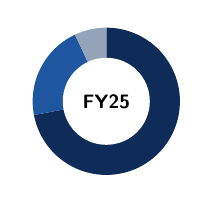
\begin{tikzpicture}[scale=0.85]
            \definecolor{pieCol1}{HTML}{0F2C59}
            \definecolor{pieCol2}{HTML}{1E56A0}
            \definecolor{pieCol3}{HTML}{94A3B8}

            \fill[pieCol1] (0,0) -- (90:1.1) arc (90:-169.2:1.1) -- cycle;
            \fill[pieCol2] (0,0) -- (-169.2:1.1) arc (-169.2:-244.8:1.1) -- cycle;
            \fill[pieCol3] (0,0) -- (-244.8:1.1) arc (-244.8:-270:1.1) -- cycle;
            \fill[white] (0,0) circle (0.65);
            \node at (0,0) {\scriptsize\textbf{FY25}};
        \end{tikzpicture}
        
        \vspace{4pt}
        \scriptsize
        \begin{tabular}{@{}ll@{}}
            \textcolor{NavyPrimary}{$\blacksquare$} Subscriptions: & 72\% \\
            \textcolor{BlueAccent}{$\blacksquare$} Token Routing: & 21\% \\
            \textcolor{TextMuted}{$\blacksquare$} Services: & 7\%
        \end{tabular}
    \end{tcolorbox}
\end{minipage}

\vspace{10pt}

% -----------------------------------------------------------------------------
% FINANCIAL MODEL & MARGIN EXPANSION
% -----------------------------------------------------------------------------
\textcolor{NavyPrimary}{\subsection*{Margin Profile \& Cash Generation Trajectory}}

\begin{minipage}[t]{0.48\textwidth}
    \vspace{0pt}
    \small
    \textbf{Operational Efficiency Gains:}
    Nexa's R\&D intensity (R\&D as \% of Revenue) is expected to normalize from 32\% in FY24 to 22\% by FY27 as foundational platform core stability is achieved. At the same time, Sales \& Marketing efficiency continues to improve due to strong inbound enterprise demand and partner co-selling.
    
    \vspace{6pt}
    \textbf{Free Cash Flow Conversion:}
    Capital expenditure requirements remain modest (CapEx < 3.5\% of Revenue) due to Nexa's asset-light cloud architecture model. We project FCF conversion from EBITDA to reach 96\% by FY27E.
\end{minipage}%
\hfill
\begin{minipage}[t]{0.48\textwidth}
    \vspace{0pt}
    \begin{tcolorbox}[calloutbox, title=\textcolor{NavyPrimary}{Operating Margin Progression (\% of Rev)}, colframe=BorderGray, colbacktitle=LightBlueBg, coltitle=NavyPrimary]
        \small
        \setlength{\tabcolsep}{3pt}
        \begin{tabularx}{\textwidth}{@{} L r r r r @{}}
            \toprule
            \textbf{Metric} & \textbf{FY24A} & \textbf{FY25E} & \textbf{FY26E} & \textbf{FY27E} \\
            \midrule
            Gross Margin & 75.8\% & 78.0\% & 79.0\% & 80.0\% \\
            R\&D / Rev & 31.5\% & 27.0\% & 24.0\% & 22.0\% \\
            S\&M / Rev & 36.2\% & 32.0\% & 28.5\% & 25.0\% \\
            G\&A / Rev & 10.1\% & 9.0\% & 8.0\% & 7.5\% \\
            \midrule
            \textbf{EBIT Margin} & \textbf{-2.0\%} & \textbf{10.0\%} & \textbf{18.5\%} & \textbf{25.5\%} \\
            \bottomrule
        \end{tabularx}
    \end{tcolorbox}
\end{minipage}

\newpage

% -----------------------------------------------------------------------------
% PAGE 3: SCENARIO ANALYSIS, RISKS & DISCLOSURES
% -----------------------------------------------------------------------------
\textcolor{NavyPrimary}{\section*{Valuation Scenario Analysis \& Sensitivity}}

\begin{tcolorbox}[calloutbox, title=\textcolor{NavyPrimary}{Bull / Base / Bear Case Breakdown}, colframe=NavyPrimary, colbacktitle=NavyPrimary, coltitle=white]
    \small
    \setlength{\tabcolsep}{4pt}
    \begin{tabularx}{\textwidth}{@{} L C C C @{}}
        \toprule
        \textbf{Scenario} & \textbf{Bull Case} & \textbf{Base Case (Our Target)} & \textbf{Bear Case} \\
        \midrule
        \textbf{Target Price} & \textbf{\$310.00} & \textbf{\$245.00} & \textbf{\$135.00} \\
        \textbf{Implied Upside / Downside} & \textcolor{BuyGreen}{\textbf{+69.9\%}} & \textcolor{BuyGreen}{\textbf{+34.2\%}} & \textcolor{BearRed}{\textbf{-26.0\%}} \\
        \midrule
        \textbf{FY25--28 Revenue CAGR} & 34.0\% & 28.5\% & 18.0\% \\
        \textbf{Terminal EBITDA Margin} & 32.0\% & 27.0\% & 20.0\% \\
        \textbf{Target EV/Sales Multiple} & 18.0x & 14.5x & 9.0x \\
        \midrule
        \textbf{Key Assumptions} & Accelerated global enterprise adoption; 140\% NRR; compute costs decline 25\% YoY. & Steady enterprise migration; 130\% NRR; linear margin expansion as modeled. & Macro IT budget freeze; increased price competition from cloud incumbents. \\
        \bottomrule
    \end{tabularx}
\end{tcolorbox}

\vspace{8pt}

\textcolor{NavyPrimary}{\subsection*{Target Price Sensitivity Matrix (WACC vs. Perpetual Growth Rate)}}

{\small
\setlength{\tabcolsep}{3pt}
\begin{tabularx}{\textwidth}{@{} L C C C C C @{}}
\toprule
\rowcolor{LightBlueBg}
\textbf{WACC \textbackslash\ Term Growth} & \textbf{2.5\%} & \textbf{3.0\%} & \textbf{3.5\% (Base)} & \textbf{4.0\%} & \textbf{4.5\%} \\
\midrule
\textbf{8.2\%} & \$268.40 & \$282.10 & \$298.50 & \$318.20 & \$342.00 \\
\textbf{8.7\%} & \$242.10 & \$253.20 & \$266.30 & \$282.00 & \$301.10 \\
\rowcolor{LightBlueBg}
\textbf{9.2\% (Base)} & \$224.50 & \$233.80 & \textbf{\$245.00} & \$258.40 & \$274.60 \\
\textbf{9.7\%} & \$209.10 & \$217.00 & \$226.20 & \$237.10 & \$250.20 \\
\textbf{10.2\%} & \$195.80 & \$202.50 & \$210.40 & \$219.70 & \$230.80 \\
\bottomrule
\end{tabularx}
}

\vspace{10pt}

\begin{minipage}[t]{0.48\textwidth}
    \vspace{0pt}
    \begin{tcolorbox}[calloutbox, title=\textcolor{NavyPrimary}{Key Investment Risks}, colframe=BorderGray, colbacktitle=LightBlueBg, coltitle=NavyPrimary]
        \small
        \begin{itemize}[leftmargin=10pt, itemsep=2pt]
            \item \textbf{Hyperscaler Competition:} Cloud providers could bundle native AI routing software into core cloud subscriptions.
            \item \textbf{Concentration Risk:} Top 10 customer accounts represent ~28\% of total subscription revenues.
            \item \textbf{Talent Acquisition Costs:} High demand for specialized engineers could inflate compensation expenses.
        \end{itemize}
    \end{tcolorbox}
\end{minipage}%
\hfill
\begin{minipage}[t]{0.48\textwidth}
    \vspace{0pt}
    \begin{tcolorbox}[calloutbox, title=\textcolor{NavyPrimary}{ESG \& Governance Overview}, colframe=BorderGray, colbacktitle=LightBlueBg, coltitle=NavyPrimary]
        \small
        \begin{itemize}[leftmargin=10pt, itemsep=2pt]
            \item \textbf{Environmental (B+):} Carbon-neutral data center routing protocols prioritize green-energy clusters.
            \item \textbf{Social (A-):} Strong employee retention rate (91\%); industry-leading data privacy standards.
            \item \textbf{Governance (A):} Independent Board Members; split CEO/Chairman structure.
        \end{itemize}
    \end{tcolorbox}
\end{minipage}

\vspace{10pt}
\hrule height 0.8pt
\vspace{6pt}

% -----------------------------------------------------------------------------
% DISCLOSURES & ANALYST CERTIFICATION
% -----------------------------------------------------------------------------
{\color{TextMuted}\tiny
\textbf{ANALYST CERTIFICATION \& IMPORTANT DISCLOSURES:} \\
The research analyst(s) named on the cover of this report certify that the views expressed accurately reflect their personal opinions about the subject securities and issuers. No part of analyst compensation was, is, or will be directly or indirectly related to the specific recommendations or views expressed herein. Meridian Capital Markets does and seeks to do business with companies covered in its research reports. As a result, investors should be aware that the firm may have a conflict of interest that could affect the objectivity of this report. Investors should consider this report as only a single factor in making their investment decision.

\vspace{2pt}
\textbf{RATING DEFINITIONS:} \\
\textbf{BUY:} Expected total return of >15\% over the next 12 months. \textbf{HOLD:} Expected total return between -5\% and +15\% over the next 12 months. \textbf{SELL:} Expected total return of <-5\% over the next 12 months.

\vspace{2pt}
Copyright \copyright\ 2026 Meridian Capital Markets. All rights reserved. Fictional sample equity research report generated for letx.app template collection. All entity names, ticker symbols, and metrics are fictional.
}

\end{document}
